\section{Ricerca di fisica Behind Standard Model con il VAEs}
\label{fisica_BSM_VAEs}

In quest'ultimo capitolo verrà presentata una possibile applicazione dei Variational Autoencoders nel campo della fisica delle alte energie, con lo scopo di ricercare segnali di nuova fisica BSM, ovvero oltre il Modello Standard. \\
Come noto, gli esperimenti portati avanti al $\textit{Large Hidron Collider}$ hanno l'obiettivo di esplorare la fisica spingendosi sempre a più alte energie; attualmente, dopo la scoperta del $\textit{Bosone di Higgs}$, la teoria del Modello Standard sembrerebbe essere completa, anche se rimango alcuni problemi aperti, come lo $\textit{Hierarchy Problem}$ e la spiegazione dell'origine della $\textit{Dark Mattern}$. \\
Nella ricerca di nuova fisica possono essere portati avanti due approcci, detti $\textit{model dependent}$ e $\textit{model independent}$. Nel primo caso la ricerca di nuova fisica avviene con un particolare modello in mente ed i risultati sono ottimi nel caso in cui il modello utilizzato è corretto, come per la scoperta del Bosone di Higgs; il limite di una ricerca di questo tipo è chiaramente dovuto al fatto che i risultati sono strettamente legati alla bontà della teoria stessa. Dall'altro lato una ricerca model independent ha il pregio di non essere legata ad una particolare teoria fisica e quindi è capace di ricercare eventuali segnali di nuova fisica a prescindere da un modello teorizzato in anticipo.\\
Nelle pagine seguenti si cercherà di capire se è possibile addestrare un Variational Autoencoder sul background in modo che sia capace di rilevare eventuali segnali di nuova fisica come anomalie. L'approccio seguito è da un lato model dependent, nel senso che i dati utilizzati sono prodotti attraverso simulazioni Montecarlo in base alla SUSY ($\textit{Supersimmetry theory}$) per la ricerca della coppia di particelle fermione/bosone (chargino e gluino), e dall'altro model independent, perché le masse di queste due particelle non sono stabilite e quindi la ricerca deve essere sensibile a tutte le varie combinazioni possibili.
\newpage

\subsection{Dataset}
\label{dataset}
Per l'addestramento del modello e per la successiva fase di verifica sono stati utilizzati i dati prodotti attraverso simulazioni Montecarlo (MC), in base alla teoria di riferimento (SUSY). I pattern prodotti in questo modo sono costituiti da otto variabili ($\textit{met}$, $\textit{mt}$, $\textit{mbb}$, $\textit{mct2}$, $\textit{mlb1}$, $\textit{lep1Pt}$, $\textit{njet30}$, $\textit{nBjet30-MV2c10}$), scelte perché sono le più discriminanti fra segnale e background per quanto riguarda la SUSY; di conseguenza lo spazio iniziale, che dovrà essere compresso e decompresso dal VAE, sarà 8-dimensionale. \\
Attraverso la simulazione MC vengono prodotti eventi sia di background che di segnale, in modo da verificare se il VAE è capace di discriminare gli uni dagli altri e, in caso affermativo, l'algoritmo potrà essere applicato a dataset reali, nei quali chiaramente non vi è questo tipo di differenziazione.\\
Prima di passare alla fase di codifica, gli eventi (sia di segnale che di background) sono stati sottoposti ad una serie di tagli di preselezione sulle variabili, come riportato nella tabella~\ref{tab:tagli di preselezione}.

\begin{table}[h!]
	\centering
	\begin{tabular}{lc}
		\hline
		&Preselezione \\
		\hline
		Esattamente un segnale di leptone&Vero\\
		met\ trigger fired&Vero\\
		$2-3$ jets con $p_{T}>30 GeV$&Vero\\
		$b$-tagged jet&[1-3]\\
		met\ &$> 220$ GeV\\
		mt\ &$> 50$ GeV\\
		mbb\ &[$100-140$]GeV\\
		mct\ &$>100$GeV\\
		\hline
	\end{tabular}
	\caption{Sono riportati i tagli di preselezione applicati sia agli eventi di segnale che a quelli di background.}
	\label{tab:tagli di preselezione}
\end{table} 
I pattern prodotti con il metodo MC sono stati divisi, come si richiede in un processo di apprendimento automatico, in una training data set, un validation data set ed un test data set.
\newpage

\subsection{Simulazione}
\label{simulazione}
Come è stato detto nelle sezioni precedenti, il VAE deve essere addestrato in modo tale da rilevare eventuali segnali di fisica BSM come delle anomalie. Ma perché un tale compito non può essere svolto da un algoritmo di apprendimento supervisionato?\\
Un semplice classificatore binario, ovvero capace di discriminare fra due sole categorie (segnale e background), viene addestrato su un training data set i cui eventi di segnale sono generati facendo riferimento ad un determinato modello; in questo modo il classificatore è in grado di discriminare solo gli eventi di segnale compatibili con quel particolare modello, tuttavia quando verranno presentati eventi di segnale prodotti con altri modelli, allora la classificazione risulterà totalmente arbitraria ed è qui che si evince il limite principale di una ricerca model dependent. \\
In linea con ciò che è già stato illustrato nel capitolo~\ref{VAEs}, gli eventi di segnale e di background, che sono stati prodotti attraverso una simulazione MC, sono rappresentabili in uno spazio 8-dimensionale. Durante il processo di addestramento del VAE i pattern relativi al background vengono compressi nello spazio latente (tridimensionale), decompressi per essere ricostruiti e poi confrontati con quelli iniziali per il calcolo dell'errore e quindi per dare il via al processo di backpropagation (~\ref{reti neurali}). \\
Nella fase di verifica si appura che l'errore nella ricostruzione dei pattern di background sia relativamente piccolo; così facendo, quando vengono presentati al VAE gli eventi di segnale, ci si aspetta che nel ricostruirli venga commesso un errore più grande e quindi la discriminazione può essere svolta osservando la distribuzione dell'errore. \\
Nel caso trattato in questa Tesi è possibile pesare in maniera diverso il contributo che le varie componenti dei pattern apportano al processo di discriminazione e, per questo motivo, verranno presentati due casi: nel primo le otto variabili avranno tutte lo stesso peso, mentre nel secondo si proverà a capire se, dando maggiore importanza ad alcune di esse, si otterrà un processo di discriminazione più efficiente. \\ 
Per prima cosa verranno illustrati i risultati ottenuti pesando tutte le variabili allo stesso modo. \\
Come primo passo bisogna capire se, a seguito del processo di addestramento, il VAE è in grado di ricostruire i pattern di background in maniera ottimale. Il risultato del processo di ricostruzione è riportato in figura~\ref{ricostruzione}. 

\begin{figure}[h!]
	\centering
	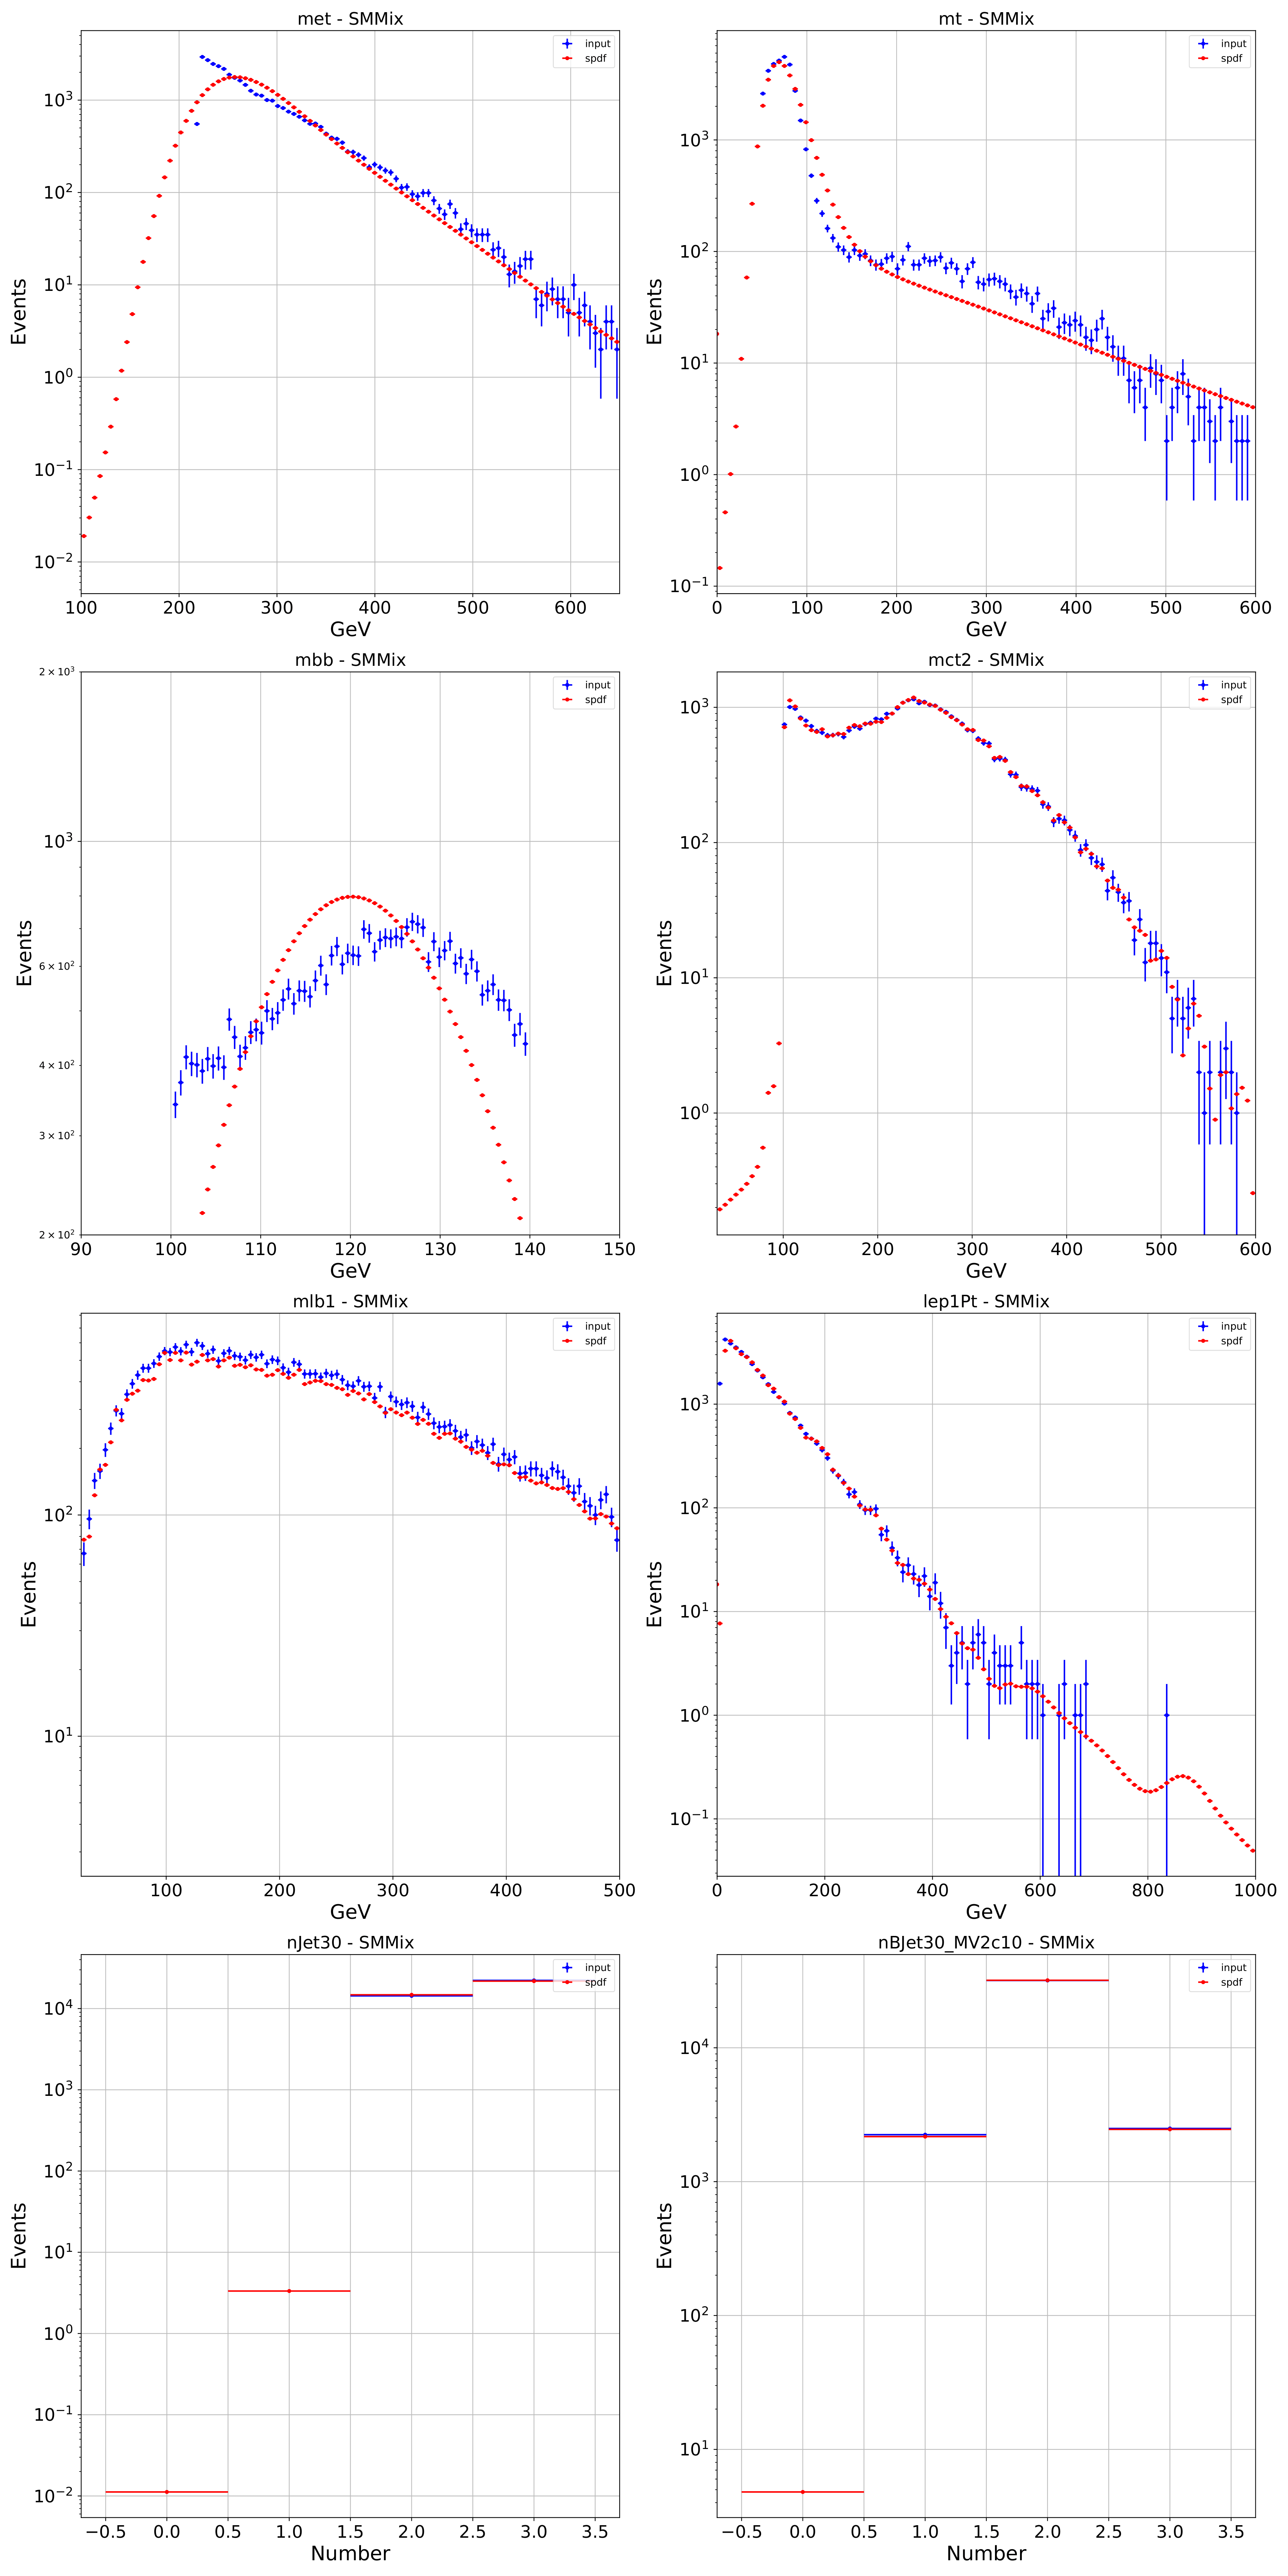
\includegraphics[width=0.75\textwidth]{figs/risultati_simulazione/ricostruzione.png}
	\caption{Confronto tra gli input in ingresso del VAE (in rosso) e quelli ricostruiti (in blu) per le otto componenti dei pattern di input.}
	\label{ricostruzione}
\end{figure}

